\begin{document}
	
	\subsection{Training}
	
	This step consist in the estimation of the centroids of the color space. May be  really time consuming, but it is performed only once, so during the actual segmentation the corresponding script isn't run.\\
	To achieved the estimation of centroids, a kmeans clustering of the multichannel images of several CT scan from different patients is performed. 
	Since to achieve a correct estimation a huge amount of scan must be provided, this task is time consuming an computational expansive, however is performed only once and isn't directly involved in the actual segmentation, so doesn't affect the segmentation time.\\
	The achievement of this task involves two main steps : 
	\begin{enumerate}
		\item \textbf{Preparation of images} : involves the building of the multi channel images, and the registration in a common space; 
		\item \textbf{Clustering} : Actual clustering, involves also the managing of the background problem.
	\end{enumerate}

		\subsubsection*{Preparation of Images} 
	
		This step involves the preparation of images, with the building of the multi channel image that incorporates neighbouring and edges informations as well as the registration in a common space and the managing of an allocation memory problem.\\
		
		First of all we have to apply a local equalization of the histogram in order to enhance the contrast between the different lung regions, after that we can start to build the multichannel image.\\		
		As I've said the multichannel image is build to incorporate more information during the clustering. We have found that a 4 channel image will provides good segmentation results. The 4 channel of the image are built as follows  : 
		\begin{itemize}
			\item Pure image after histogram equalization; 
			\item Median Blurred of the equalized image; 
			\item standard deviation map of the pure image
			\item Maximum eigenvalues map 
		\end{itemize}
	
		\begin{figure}[h]
			\centering
				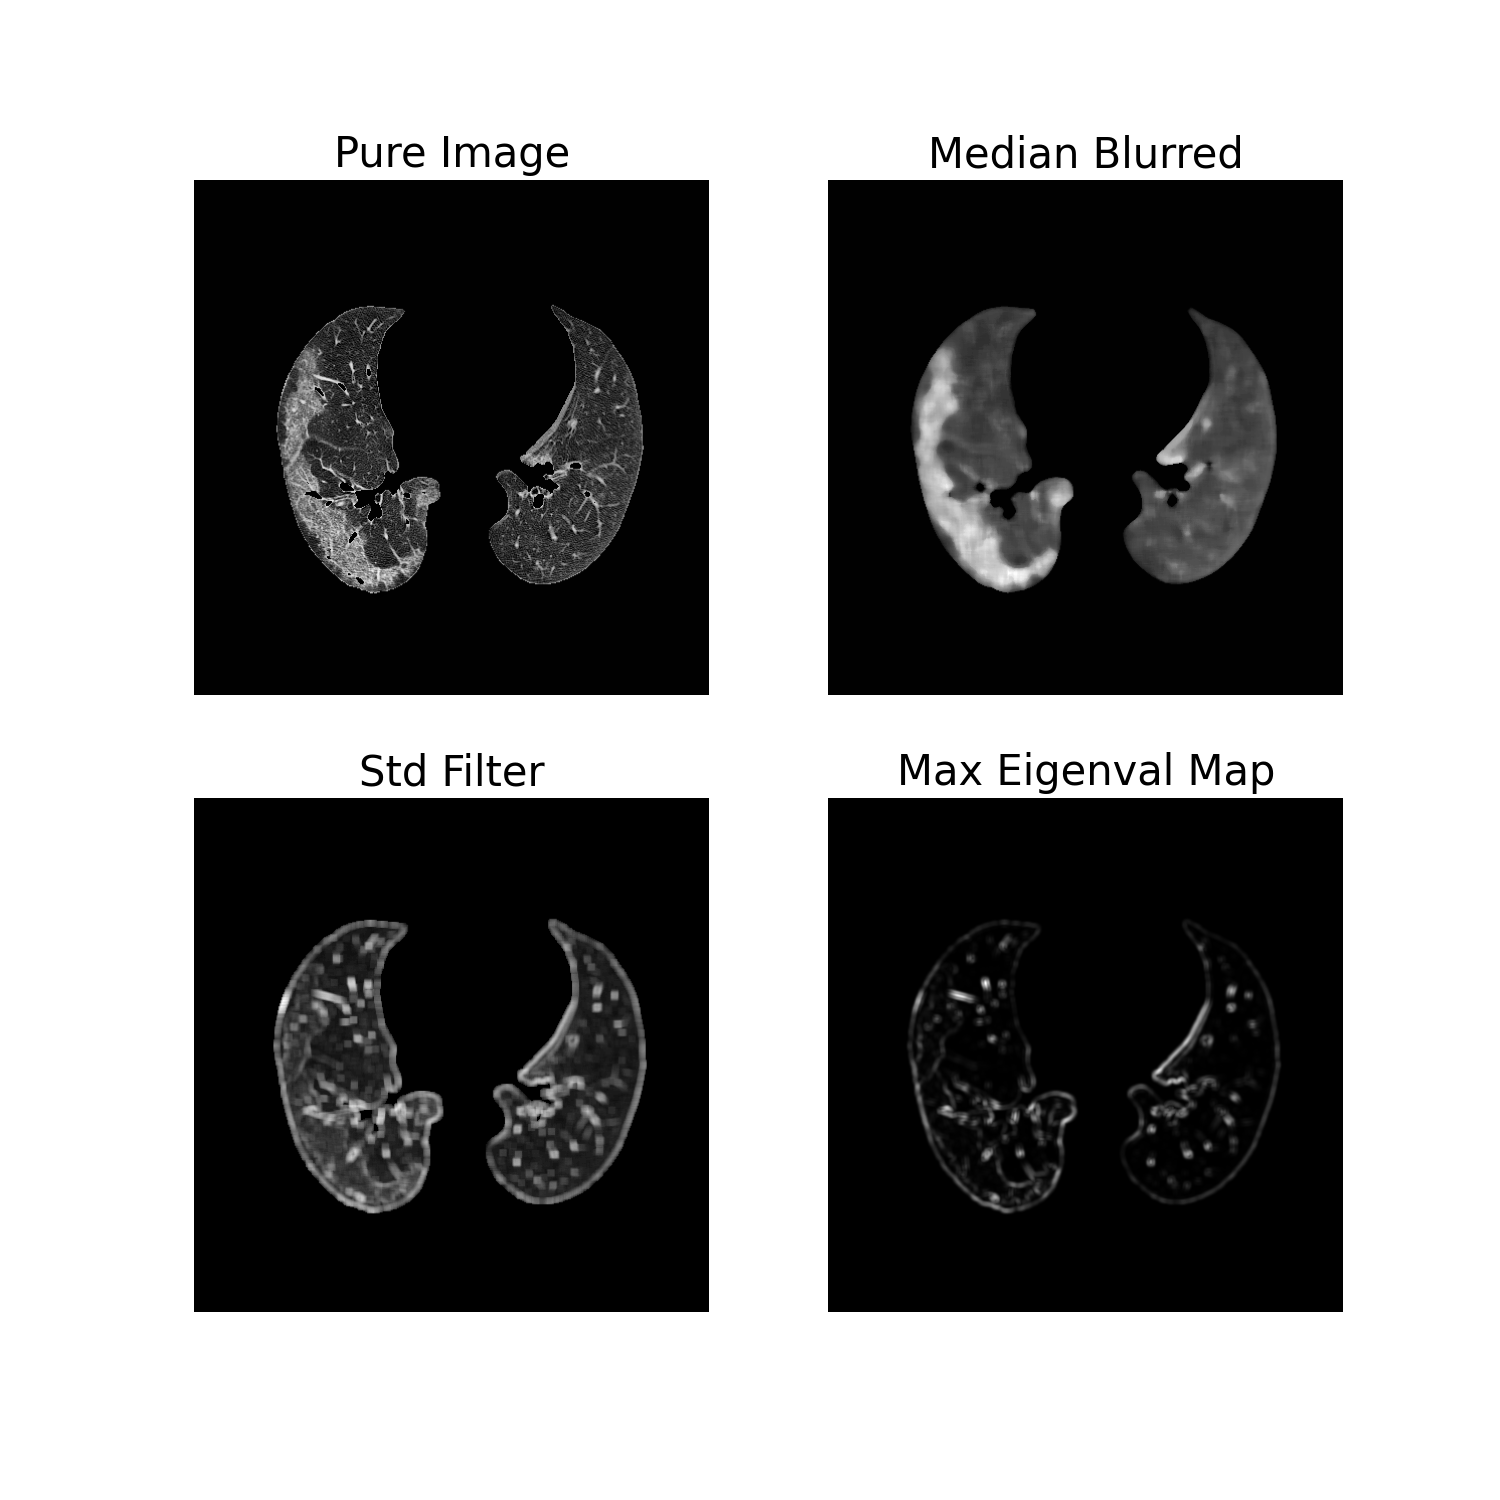
\includegraphics[scale=.55]{Multi_Channel.png}
			\caption{Image used for each dimension of the color space from left to right and from top to bottom we have the pure image, the median blurred image, the std filtered and the maximum eigenvalues map.}\label{fig:MultiChannel}
		\end{figure}
	
		In \figurename\,\ref{fig:MultiChannel} I've displayed the 4 different channel of the image. Each channel allow us to consider different information:\\ 
		The pure image will provides information about the tissue displayed in the single voxel; 
		The median blurred image allow us to consider also information about the tissue surrounding each particular voxel, since lesions usually involves several group of voxels.\\ The maximum eigenvalues map allow us to consider also shape information. A source of error was the remaining bronchial structures and  motion artifacts. Usually this features have a thin and elongated shape, in contrast with the lesion areas which are less thin or less elongated. Elongated structures presents an eigenvalues higher than the other. on the other hand rounded structure presents eigenvalues more or less equal. This map allow us to discriminate between actual lesion regions and bronchial structures and motion artifacts.  In this way we are able to reduce the false positives caused by this kind of artifacts. In the end the standard deviation map, which consist in the replacement of each pixel value with the standard deviation of its neighborhood, help us, like the maximum eigenvalues map, to distinguish the bronchial and artifact structures.
		
		The first step consist into the construction of the multichannel image of for each input series, after that all the images are shuffled and divided into several sub-samples. The creation of several sub-samples is made since the creation of a single, huge array with several images is not always possible, since requires a huge quantity of memory to be allocated, so we have chose to divide all the images into several sub-samples and cluster them independently, after that a clustering on the estimated centroids is performed.\\

		
		\subsubsection*{Clustering} 
		
		This step consist into the performing of the kmeans clustering for the centroids estimation. To perform this task I've used the OpenCV algorithm, which provides an optimized implementation of the algorithm for multi channel images. A first clustering is applied on each sub-sample, resulting in a set of centroids for each one of them. On this set is applied a second clustering, which provides the actual centroids. In both of the clustering, the initial centroids set is initialized by using the kmeans ++ algorithm, which allows to improve speed and accuracy of the clustering algorithm~\cite{Arthur2007}.
		During this task we have to manage some issues. As we can see from \figurename\,\ref{fig:ClusteringHistogram} the number of voxel with $GL = 0$  is several order of magnitude higher than for other $GL$. As prior we know that these voxels belonging from background, so this cluster is over represented. Since kmeans cluster requires an homogeneous representation for each cluster, this may raise problem during the centroids estimation. In order to overcome this issue we have simply removed this voxels from the clustering.  
		

		\begin{figure}[h!]
			\centering
				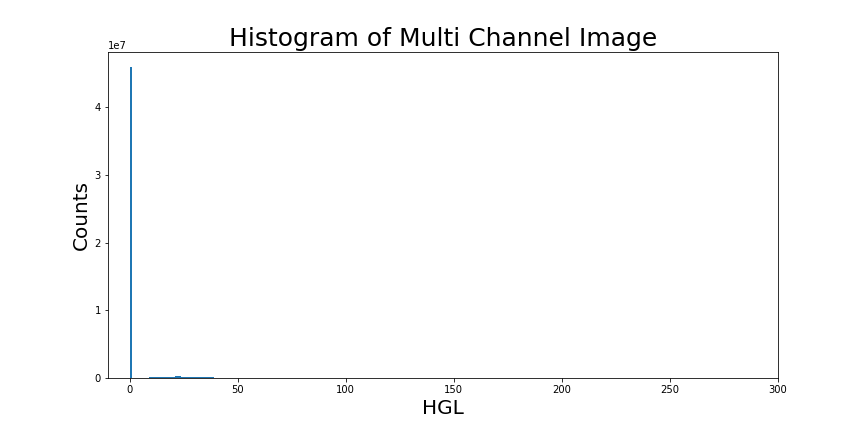
\includegraphics[scale=.5]{HistMC.png}
				\caption{Histogram of the multichannel image to cluster, we can clearly see the overrepresented cluster at $0$ GL}	\label{fig:ClusteringHistogram}
		\end{figure}
		
	An other problem may be the estimation of the correct number of clusters. Kmeans clustering requires a prior knowledge on the number of clusters which is a crucial choice. In our case the anatomical knowledge about the lung may help, since we can consider one cluster for each anatomical structure. In the end we have found that 5 clusters are an optimal choice, and the considered structures are the following: 
	\begin{itemize}
		\item Lung Parenchima;
		
		\item Edges;
		
		\item vessel surrounding bronchial structures;
		
		\item Ground Glass Opacities and consolidation;
		
		\item Bronchi.

	\end{itemize}

	
	We don't need a cluster to represent the background, since as I' ve said before the corresponding voxel aren't takes into account during the clustering.\\
	In the end a set of centroids for each subsamples was estimated and a second clustering was performed, to found the optimal centroids. 
	This process takes a lot of time, but once we have estimated the optimal centroid set, we haven't to repeat it.\\
	
	The pseudocode of this script is reported in algorithm\,\ref{alg:training}
		
		
	\begin{algorithm}
	
	\SetAlgoLined
	\DontPrintSemicolon
	
	\SetKwFunction{FSub}{shuffle\_and\_split}
	\SetKwFunction{Fk}{kmeans\_on\_subsamples}
	\SetKwProg{Fn}{Function}{:}{}
	
	\Fn{\FSub{$images,\, number of subsamples$}}{{
	
			images$\leftarrow$shuffle(images)\;
			output$\leftarrow$split(images, number of subsamples )\;
		}
		\textbf{return} $ output $ 
	}
	\textbf{End Function}

	\Fn{\Fk{$subsamples,\, number of centroids$}}{{
			
			centroids <- []\;
			\ForEach{$ Sub \in subsamples $}
			{
				center$\leftarrow$kmeans(sub, number of centroids)\;
				centroids$\leftarrow$append(center)
				
			}
		
		}
		\textbf{return} $ centroids $ 
	}
	\textbf{End Function}
	
	\KwData{CT scans with Extracted lung}
	\KwResult{Centroid matrix}
	
	\ForEach{$scan \in input\_scans$}{
	
		read the scan\;
		sample$\leftarrow$image\_array\;
	}

	sample$\leftarrow$ build\_multichannel(sample)\;
	subsamples$\leftarrow$shuffle\_and\_split(sample, number of subsamples)\;
	centroid\_vector$\leftarrow$kmeans\_on\_subsamples(subsamples, n\_centroids)\;
	centroid$\leftarrow$kmeans\_clustering(centroid\_vector, n\_centroids)\;
	
	\caption{Pseudo-code for the training script}\label{alg:training}
	
\end{algorithm}

	
\end{document}